% !TEX encoding = UTF-8
% !TEX TS-program = pdflatex
% !TEX root = ../tesi.tex

%**************************************************************
\chapter{Progettazione e codifica}
\label{cap:progettazione e codifica}
%**************************************************************

\intro{In questo capitolo vengono approfondite approfondite la progettazione e la codifica. La progettazione entra nel dettaglio dell'architettura, delle viste progettate e delle API, mentre la codifica descrive il processo di sviluppo dei principali componenti e service dell'applicazione.}\\

\section{Progettazione}
\subsection{Architettura Angular}
Un'applicazione Angular è formata da un insieme di moduli, dove il modulo pricinpale è il modulo root, chiamato AppModule, che contiene più moduli di funzionalità. Un modulo di funzionalità è composto da un componente, che definisce la vista dell'utente.\\
Ogni componente possiede un template HTML, che definisce la struttura della vista e i vari eventi che può emettere. Ogni evento emesso, se gestito, può modificare lo stato interno del componente, che si riflette nella struttura HTML e in fine scatena l'aggiornamento della vista.\\
% Quindi un click su un bottone questo elemento HTML emette un evento di click al componente in cui si trova, questo componente esegue il metodo specifico al evento ricevuto, di seuito viene cambiato il metadata e viene aggiornato il template di HTML.\\
I componenti utilizzano dei servizi che forniscono funzionalità specifiche come il login di Auth.Service, ma non sono correlate direttamente alla vista, essi sono inseriti come delle dipendenze, potenzialmente in più componenti e questo rende tali servizi modulari. Non solo i servizi sono riutilizzabili ma anche i componenti lo sono, dunque rende l'applicazione Angular più semplice da comprendere e manutenibile in futuro.\\
\begin{figure}[H]
    \centering
    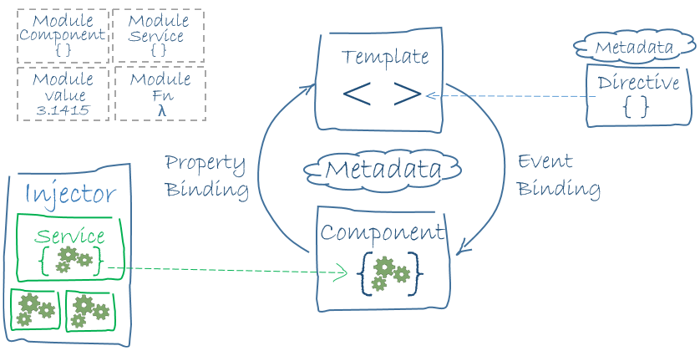
\includegraphics[scale=0.5]{angularArc.png}
    \caption{Architettura Angular}
\end{figure}
\subsection{Architettura SushiLab}
La web-app segue l'architettura spiegata precedentemente che è anche quella consigliata dal sito ufficiale di Angular.\\
La cartella principale della del progetto è "app/" che contiene tutti i componenti, i servizi e il root.\\ 
Per ogni componente è stata creata una cartella apposita, che contiene i file .ts per la logica, .html per la struttura, .scss per lo stile e infine i suoi componenti figli. Per i componenti condivisi si è creato una cartella shared dove vengono salvati i componenti che sono utilizzati in più parti dell'applicazione.\\
Nella cartella REST vengono salvati tutti i file service, in cui ci sono dei metodi che vengono chiamati in più componenti dell'applicazione al fine di massimizzare il riuso del codice.\\
Nella cartella assets vengono salvati le immagini e le icone utilizzate, in modo da fare utilizzare da tutti i componenti.\\
\begin{figure}[H]
    \centering
    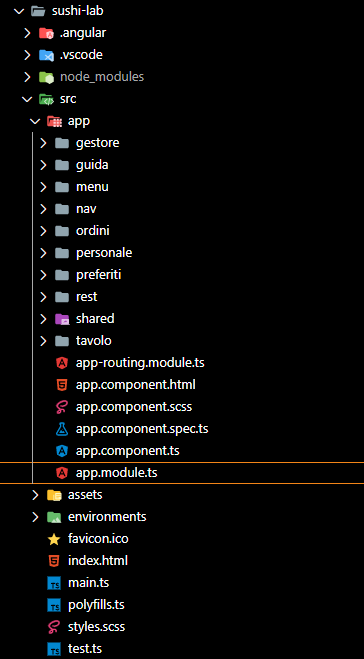
\includegraphics[scale=0.55]{struttura.png}
    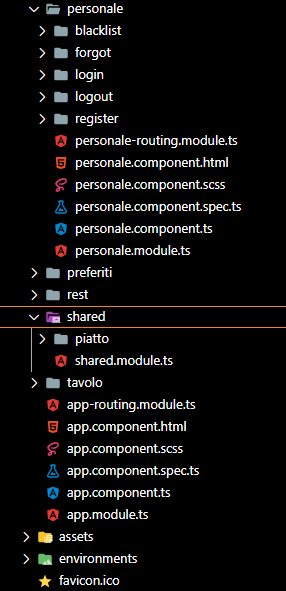
\includegraphics[scale=0.6]{struttura1.png}
    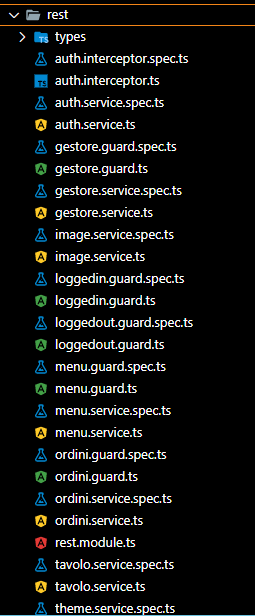
\includegraphics[scale=0.55]{struttura2.png}
    \caption{Struttura file SushiLab}
\end{figure}
\subsection{Progettazione delle viste}
All'inizio si è fatto un meeting con il tutor aziendale per chiarire le funzionalità e i requisiti che la web-app deve avere, dopo di che si è iniziato la progettazione dei \gls{mockg} delle viste tramite la editor di grafica online Figma.\\
Tramite il sistema di progettazione di Figma sono stati creati le bozze delle viste per chiarire i collegamenti tra di loro e i posizionamenti dei compoenti. 
Il posizionamento è scelto in base alla frequenza di click su di essa e si basa anche sulle viste dei web-app più popolari.
È stato deciso i seguenti aspetti:
\begin{itemize}
    \item I colori principali e lo sfondo della applicazione;
    \item Il bottone per la navbar è in alto a destra;
    \item Il logo della piattaforma in alto a sinistra;
    \item I bottoni, testi e form devono avere lo stesso stile e colore in base alla loro funzionalità;
    \item Lo stile del piatto in modalità dettaglio in menù e nella lista degli ordini personali è la stessa.
\end{itemize}
\begin{figure}[H]
    \centering
    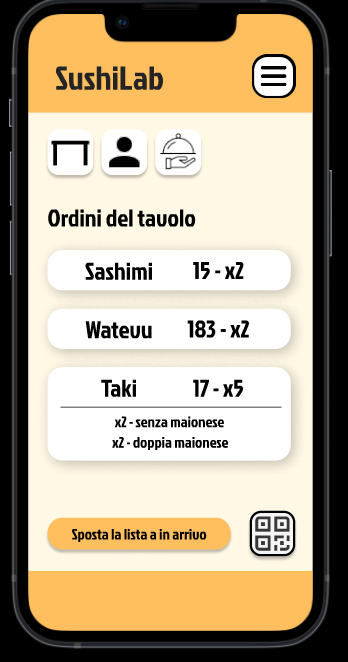
\includegraphics[scale=1]{figma.png}
    \caption{Figma SushiLab}
\end{figure}
\subsection{Progettazione API}
Durante il periodo di stage non era ancora presente il back-end per l'applicativo, quindi si è deciso con l'azienda di progettare dei mock API per il testing utilizzando la piattaforma Stoplight.\\
La progettazione delle API sono molto semplici grazie all'interfaccia semplice di Stoplight, che permette di definire i path e i rispettivi metodi facilmente, e ai mock-up delle viste prima definite.\\
Per ogni chiamata REST bisogna definire:
\begin{itemize}
    \item \textbf{Nome:} individua API;
    \item \textbf{Descrizione:} spiega in dettaglio la funzione della API;
    \item \textbf{Metodo:} definisce il tipo di chiamata, è stato usato:
    \begin{itemize}
        \item  \textbf{get:} per richiedere dei dati al server come la chiamata per ottenere il menù;
        \item  \textbf{post:} per inviare dei dati sintetici al server come i dati per login;
        \item  \textbf{delete:} per eliminare dei dati dal server come eliminazione della sessione di tavolo.
    \end{itemize}
    \item \textbf{Path:} definisce il percorso finale della API;
    \item \textbf{Risposta:} configura la risposta che ritorna la API, è stato usato:
    \begin{itemize}
        \item  \textbf{200:} richiesta andata a buon fine;
        \item  \textbf{201:} creazione andata a buon fine;
        \item  \textbf{204:} richiesta andata a buon fine ma il contenuto è vuoto;
        \item  \textbf{401:} non autorizzato;
        \item  \textbf{404:} non trovato;
        \item  \textbf{406:} non accettato;
        \item  \textbf{500:} errore interno.
    \end{itemize}
\end{itemize}
\begin{figure}[H]
    \centering
    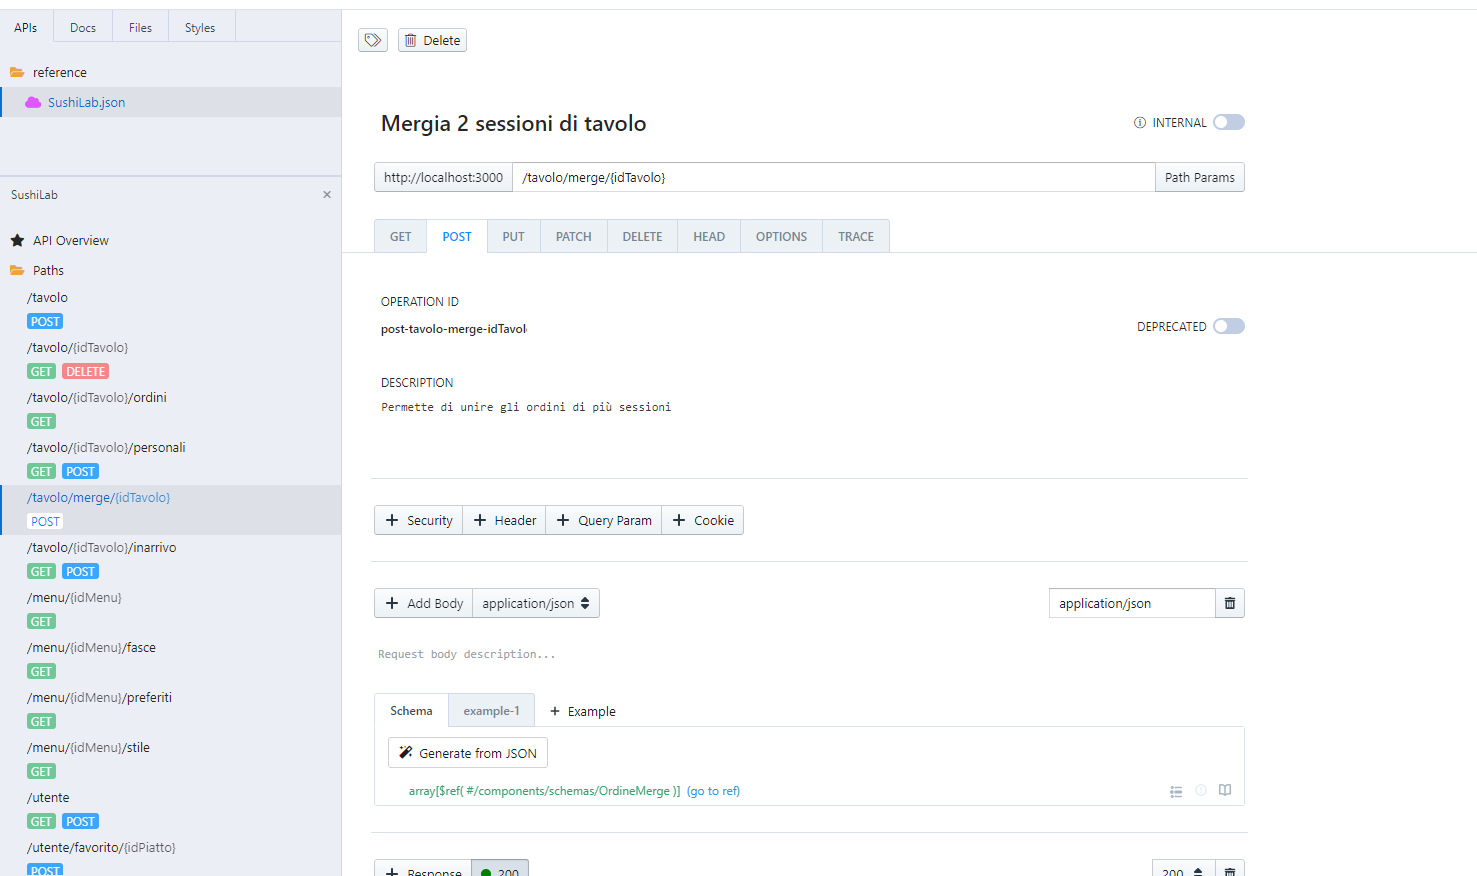
\includegraphics[scale=0.55]{stoplight.png}
    \caption{Stoplight SushiLab}
\end{figure}

\subsection{Progettazione dei componenti}
I componenti sono stati individuati tramite l'analisi dei requisiti e la progettazione delle viste. Ogni componente ha delle funzionalità specifiche e tutti assieme costruiscono la web-app, coprendo tutti i requisiti richiesti.
\\
% {\hyperref[cap:menu.component]{Il secondo capitolo}}
\section{Codifica}
\subsection{Interfacce}
Dopo aver progettato i mock della visuale tramite figma e le API tramite stoplight ho iniziato la fase di codifica delle interfacce. La creazione dei template di default dei componenti è stata molto rapida grazie al command-line interface di Angular, utilizzando il comando 'ng generate component "nome del componente"' che crea una cartella contenente tutti i file necessari per il rendering del componente. Dopo la creazione dei file principali ho proceduto a modificare il component.ts, che rapprensenta la logica del componente, inserendo tutte le funzionalità che il componente deve avere. Una volta definito questo sono passato alla struttura e allo stile, quindi a modificare il component.html e il component.css.
Tutte le interfacce, con le loro funzionalità e una descrizione dettagliata, possono essere reperite nell'appendice {\hyperref[cap:appendice c]{C}}.
\subsubsection{Componenti service}
Per la comunicazione e gestione dei vari componenti vengono adoperati i file service. Per ogni servizio viene creato un file.service utilizzabile da uno o più component.\\
I servizi utilizzati sono:
\begin{itemize}
    \item auth.service: per gestire le autenticazioni;
    \item menu.service: per gestire tutte le funzionalità del menù;
    \item ordini.service: per gestire le ordinazioni;
    \item tavolo.service: per gestire le sessioni di tavolo;
    \item user.service: per gestire le funzionalità dell'area personale.
\end{itemize}
\subsubsection{Componenti guard}
Arrivato alla fine della codifica si definiscono i componenti guard, che permettono di imporre delle regole di accesso per la navigazione in un determinato componente. La verifica delle regole di guard avviene all'interno del metodo canActivate, appogiandosi ai diversi service e ai dati locali di sessione.